\chapter{Heuristic Algorithm}

Exact methods are algorithms that guarantee an optimal solution to a given problem will be found.
A very crude example is exhaustive (brute-force) search, which systematically enumerates all candidate solutions.
For linear problems, simplex algorithm, interior-point methods, and branch and bound are often used~\cite{HMO/ExactMethods}.
If $\text{P} \neq \text{NP}$, this NP-hard optimization problem cannot be optimally solved in worst-case polynomial time.

When an optimal solution is not required, or the optimization problem is intractable and an exact algorithm cannot solve it in reasonable time, heuristic algorithms may be used.
They do not offer any guarantees with respect to solution quality, but often find satisfying solutions in polynomial time.
Heuristic algorithm are divided into constructive algorithms, which gradually build a solution piece by piece, and improvement algorithms, which start from an existing solution and incrementally improve it~\cite{Cupic/Metaheuristics}.

A metaheuristic algorithm is a kind of general-purpose heuristic algorithm, with the task of guiding problem-specific heuristics towards parts of the solution space which contain high-quality solutions~\cite{Cupic/Metaheuristics}.
They are often inspired by processes occurring in nature.
Examples include tabu search, ant colony optimization algorithms, particle swarm optimization, genetic algorithm, and other evolutionary algorithms.
Metaheuristic algorithms are divided into algorithms which operate on a single solution, and those that operate on a set of solutions (population-based algorithms).

Herein, we describe the heuristic algorithm for aerial resource scheduling proposed in this thesis.


\section{Schedule Representation}

We define a \textit{takeoff} as a 3-tuple consisting of an aerial resource, a fire front, and a time slot, in that order: $(k, f, t)$.
It indicates that the aircraft $k$ is departing in the time slot $t$ in order to fight the fire at the front $f$.
In the pseudocode, a takeoff is typically given the name $e$, short for \textit{element}.

A \textit{schedule} is represented by a set of \textit{takeoffs}.
It is a one-to-one mapping of the model's decision variable, i.e., the takeoff matrix and its elements \hbox{$c_{kf}^t \in \left\{ 0, 1 \right\}$}:
\begin{equation}
    (k, f, t) \in \mathit{Schedule} \iff c_{kf}^t = 1,\ \forall k \in \mathcal{K}, f \in \mathcal{F}, t \in \mathcal{T}
\end{equation}

If a set of takeoffs does not satisfy all the constraints, it is not considered to be a valid schedule.
Because of the way the model and constraints are defined, every subset of a valid schedule is also a valid schedule, including an empty set.
Recall, the water target is a soft constraint moved to the objective function.
Thus, solutions which do not meet the desired water target are considered valid solutions as long as they satisfy the remaining constraints (availability, legislation, etc.). 
Furthermore, once a schedule becomes invalid by adding a takeoff which breaches a constraint, it is impossible to bring it back to a valid state by inserting more takeoffs.
Therefore, we limit ourselves to operating exclusively on valid schedules throughout the heuristic algorithm.
In order for a takeoff to even be considered for insertion into a schedule (referred to as potential or feasible takeoffs), the result must be a valid schedule.

The terms \textit{schedule} and \textit{solution} are used interchangeably.
In the pseudocode, they are sometimes given the short name $s$.

Consider a large problem instance with $7\,000$ different takeoffs, and a maximum of $100$ takeoffs in a schedule.
The upper limit on the number of different schedules is $\binom{7\,000}{100} \approx 1.7 \cdot 10^{226}$.
Obviously, the majority of those schedules are invalid, but that still easily puts the size of the search space above $10^{200}$ different valid solutions.


\section{Greedy Randomized Adaptive Search Procedure}

\begin{algorithm}[tb]
    \caption{Greedy Randomized Adaptive Search Procedure}
    \label{alg:grasp}
    
    \newcommand{\Stemp}{s'}
    \newcommand{\Sbest}{s^{\mathrm{best}}}
    
    \begin{algorithmic}[1]
        \Procedure{GRASP}{$\mathit{iterations}, N_D, N_R, \alpha_G, \alpha_D, \alpha_R, k_{r, G}, k_{p, G}, k_{r, R}, k_{p, R}, T_0, \beta, L$}
            \State $\Sbest \gets \emptyset$\,;
            \For{$i \gets 1$ \textbf{to} $\mathit{iterations}$} \label{alg:grasp-line-for-loop}
                \State $s \gets$ \Call{ConstructGreedySolution}{$\alpha_G, k_{r, G}, k_{p, G}$};
                \State $\Stemp \gets$ \Call{LocalSearch}{$s, N_D, N_R, \alpha_D, \alpha_R, k_{r, R}, k_{p, R}, T_0, \beta, L$};
                \If{$f(\Stemp) > f(\Sbest)$} \label{alg:grasp-line-if-better}
                    \State $\Sbest \gets \Stemp$;
                \EndIf
            \EndFor
            \State \textbf{return} $\Sbest$;
        \EndProcedure
    \end{algorithmic}
\end{algorithm}

The \textit{greedy randomized adaptive search procedure} (GRASP) is a multi-start metaheuristic algorithm, first introduced in Ref~\cite{Feo/GraspFirst}.
Each iteration or independent start consists of two phases -- initial construction, and local search~\cite{Feo/GraspReview}.
The construction phase employs a randomized greedy approach which most often starts with an empty solution.
Local search is then applied to improve upon the initial solution.
The two phases are otherwise not related, and exact algorithms for each phase can be chosen and modified practically without restrictions.
However, the search is required to be stochastic, as there is no sense in executing a deterministic algorithm more than once.
In the proposed algorithm, both phases are stochastic.

The GRASP pseudocode is shown in Algorithm~\ref{alg:grasp}.
The function takes a large number of parameters, all of which will be explained in later sections, where they are used.

Because of complicated constraints, especially the one stating that different types of aircraft cannot fly at the same front at the same time, it is easy for the search to drift in a certain direction and end up with parts of the solution that hardly ever change.
As an example, some schedule might have only airplanes flying at the fire front $f$ during the first half of the day, when it would have been better for them to be flying at a different front, or at $f$ but in the afternoon.
Making such a switch during local search can be extremely unlikely, particularly if it was not considered when designing the algorithm.
GRASP is the metaheuristic of choice because restarting the search often leads to vastly different initial solutions, some of which will hopefully nudge local search in a different direction.
Moreover, it can be seen that iterations have no search memory, making them almost completely independent from one another, except for the result aggregation phase (line~\ref{alg:grasp-line-if-better}).
This makes the algorithm trivially parallelizable, which is another reason why GRASP was selected.


\section{Randomized Greedy Algorithm}

\begin{algorithm}[tbp]
    \caption{Greedy Solution Construction}
    \label{alg:greedy}
    
    \newcommand{\Solution}{\mathit{Solution}}
    
    \begin{algorithmic}[1]
        \Procedure{ConstructGreedySolution}{$\alpha_G, k_{r, G}, k_{p, G}$}
            \State $\Solution \gets \emptyset$\,;
            \State $C \gets$ Candidate set of all feasible takeoffs in $\Solution$;
            \While{$C \not= \emptyset$} \label{alg:greedy-line-while-nonempty}
                \State $\Solution \gets$ \Call{GreedilyInsertTakeoff}{$\Solution, \alpha_G, k_{r, G}, k_{p, G}$};
                \State Update $C$ with respect to constraints;
            \EndWhile
            \State \textbf{return} $\Solution$;
        \EndProcedure

        \State

        \Procedure{GreedilyInsertTakeoff}{$s, \alpha_G, k_r, k_p$}
            \State $\Solution \gets s$;
            \State $C \gets$ Candidate set of all feasible takeoffs in $\Solution$;
            \If{$C = \emptyset$} \label{alg:greedy-line-check-empty}
                \State \textbf{return} $\Solution$;
            \EndIf

            \State $o(e) \gets$ Objective function value for $\Solution \cup \{ e \}$; \label{alg:greedy-line-o-def}

            \State $r(e) = \left\vert \left\{ e' \in C \, \mid \, e'.k = e.k \right\} \right\vert$; \label{alg:greedy-line-r-def}

            \State Calculate available takeoffs if $e$ were chosen next: $C_e$ for all $e \in C$;
            \State $p(e) = \left\vert C_e \right\vert$ for all $e \in C$; \label{alg:greedy-line-p-def}
            
            \State Evaluate $o(e)$, $r(e)$, $p(e)$ for all $e \in C$;

            \State $\hat{o} \gets$ Linearly scaled $o$ to range $\left[ 0, 1 \right]$;
            \State $\hat{r} \gets$ Linearly scaled $r$ to range $\left[ 0, 1 \right]$;
            \State $\hat{p} \gets$ Linearly scaled $p$ to range $\left[ 0, 1 \right]$;

            \State Evaluate the fitness function:
            \State ~~~~$f(e) = \hat{o}(e) - k_r \cdot \hat{r}(e) + k_p \cdot \hat{p}(e)$ for all $e \in C$; \label{alg:greedy-line-fitness-def}

            \State $\mathit{f^{min}} \gets \min \{f(e) \, \mid \, e \in C \}$;
            \State $\mathit{f^{max}} \gets \max \{f(e) \, \mid \, e \in C \}$;
            \State $\mathit{RCL} \gets \left\{e \in C \, \mid \, f(e) \ge f^{max} - \alpha_G \left( f^{max} - f^{min} \right) \right\}$; \label{alg:greedy-line-rcl}
            \State Randomly select $\mathit{Takeoff}$ from $\mathit{RCL}$;

            \State $\Solution \gets \Solution \cup \{ \mathit{Takeoff} \}$;
            \State \textbf{return} $\Solution$;
        \EndProcedure
    \end{algorithmic}
\end{algorithm}

A randomized greedy algorithm is used in the first phase of GRASP.
Its pseudocode is given in Algorithm~\ref{alg:greedy}.
It is a constructive algorithm, meaning that it starts from an empty solution and gradually inserts elements into it.
Construction stops when there are no more elements which can be inserted (line~\ref{alg:greedy-line-while-nonempty}).

The element to be inserted in each iteration is randomly chosen from a \textit{restricted candidate list} (RCL), a concept first described in Ref~\cite{Hart/RCL}.
All candidate elements, i.e., feasible takeoffs, are evaluated based on a fitness function.
A threshold is calculated based on the value of the parameter \hbox{$\alpha_G \in [ 0, 1 ]$}, as shown in line~\ref{alg:greedy-line-rcl}.
Because we are dealing with a maximization problem, only the takeoffs with the fitness value higher or equal to the threshold enter the restricted candidate list.
If the value of $\alpha_G$ is $0$, the best takeoff is selected every time, and the algorithm is completely deterministic.
If the value is $1$, the selection is completely random.

Instead of using the parameter $\alpha_G$ and the threshold, the RCL could be defined by taking a predefined number of elements with the highest fitness value.
It was decided not to use this approach because the quality of the solution can vary quite a lot for instances of different sizes if the same number is used.
For example, picking ten elements out of a thousand can be too restrictive, while picking ten out of twenty can be too random.
On the other hand, selecting the best $5\%$ of elements ($\alpha_G = 0.05$) should give mostly consistent results regardless of instance size.

The fitness function $f(e)$ is not the same as the objective function.
Instead, a weighted combination of three metrics is used in order to measure the benefit of selecting each takeoff.
The metrics are designed so that the choice of a takeoff in one iteration does not severely limit the choices available in the subsequent iteration, which is effectively limiting the greediness.

The first metric $o(e)$ (line~\ref{alg:greedy-line-o-def}) calculates the value of the objective function for the solution if takeoff $e$ were inserted.
It does not have an explicit weighting factor associated with it, as it is considered to be a baseline with the implicit factor $1$.

The second metric is the function $r(e)$, defined in line~\ref{alg:greedy-line-r-def}.
It counts the number of distinct potential takeoffs for the same aerial resource as the one in takeoff $e$.
Takeoffs with a lower value are preferred because related aircraft have fewer takeoffs left to choose from.
In later stages the choice will probably be further reduced, as other inserted takeoffs might block previously available takeoffs.
The value is scaled by a non-negative weighting factor $k_r \in \mathbb{R}^+$.

The third metric is $p(e)$ (line~\ref{alg:greedy-line-p-def}), used to count what would be the total number of feasible takeoffs in the next iteration if takeoff $e$ were selected in this iteration.
Higher values are considered better because they mean selecting that takeoff makes less of a difference with respect to limiting the number of choices in the future.
The value is scaled by a non-negative weighting factor $k_p \in \mathbb{R}^+$.

In order to avoid issues with different scales of different metrics, each of them is scaled to the range $[0, 1]$.
The importance of a metric is then determined only by the assigned weighting factor.
All of the metric are combined into the fitness function in line~\ref{alg:greedy-line-fitness-def}.

The candidate takeoffs need to be re-evaluated in every iteration because the benefits associated with every takeoff change when another is added to the solution.
The candidate set can also drastically change, as the insertion of one takeoff can make dozens of others infeasible.

The check in line~\ref{alg:greedy-line-check-empty} is redundant in the construction phase because of the condition in line~\ref{alg:greedy-line-while-nonempty}.
However, it will be relevant when the same procedure is reused as a part of local search is Section~\ref{sec:repair}.


\section{Local Search}

\textit{Local search} (LS) aims to improve the solution previously found during the greedy construction phase.
It is an improvement algorithm, meaning that it starts with a valid solution and iteratively attempts to find another solution with a higher objective function value, usually stopping when a local optimum is found~\cite{Feo/GraspReview}.
A solution is locally optimal if there is no other solution in the neighborhood with a higher value of the objective function (for a maximization problem).
A neighborhood of a solution is the set of valid solutions which can be reached from the current solution by performing a \textit{move} operation~\cite{Cupic/Metaheuristics}.
The design of those operations plays a vital role in the performance of the algorithm.

The pseudocode is given in Algorithm~\ref{alg:localsearch}.
In the proposed heuristic algorithm, local search is implemented as a combination of large neighborhood search and simulated annealing.
Large neighborhood search is used to sample a single solution $s'$ from the neighborhood (lines~\ref{alg:localsearch-line-destroy} and \ref{alg:localsearch-line-repair}).
Simulated annealing is then used to determine if the sampled solution should be accepted as the current solution $s$ (lines~\ref{alg:localsearch-line-sa-start}~--~\ref{alg:localsearch-line-sa-end}).
Both algorithms are explained in detail in upcoming sections.
Every sampled solution $s'$ is compared to the incumbent solution $s^{\mathrm{best}}$ (line~\ref{alg:localsearch-line-if-best}), which is updated if necessary.

There can be a number of different reasons why the search would be terminated, commonly named stopping criteria.
For example, the time limit is exceeded, the number of iterations without improvement of the incumbent solution is reached, or a local optimum is found.
Because the neighborhood is not exhaustively searched in this version of local search, it is not possible to say with certainty if a local optimum was reached.
Instead, the search is stopped when the total number of iterations, $L$, is reached.

\begin{algorithm}[tb]
    \caption{Local Search}
    \label{alg:localsearch}
    
    \newcommand{\Stemp}{s'}
    \newcommand{\Sbest}{s^{\mathrm{best}}}
    
    \begin{algorithmic}[1]
        \Procedure{LocalSearch}{$s, N_D, N_R, \alpha_D, \alpha_R, k_{r, R}, k_{p, R}, T_0, \beta, L$}
            \State $\Sbest \gets s$;
            \State $T \gets T_0$; \label{alg:localsearch-line-temp-init}
            \For{$i \gets 1$ \textbf{to} $L$}
                \State $s_D \gets$ \Call{Destroy}{$s, N_D, \alpha_D$}; \label{alg:localsearch-line-destroy}
                \State $\Stemp \gets$ \Call{Repair}{$s_D, N_R, \alpha_R, k_{r, R}, k_{p, R}$}; \label{alg:localsearch-line-repair}
                \If{$f(\Stemp) > f(\Sbest)$} \label{alg:localsearch-line-if-best}
                    \State $\Sbest \gets \Stemp$;
                \EndIf
                
                \State $\Delta f =  f(\Stemp) - f(s)$; \label{alg:localsearch-line-sa-start}
                \If{$\Delta f > 0$\, \textbf{or}\, $\mathrm{rand}(0, 1) < e ^ {\Delta f / \, T}$} \label{alg:localsearch-line-sa-accept}
                    \State $s \gets \Stemp$;
                \EndIf
                
                \State $T \gets \beta \cdot T$; \label{alg:localsearch-line-sa-end}
            \EndFor
            \State \textbf{return} $\Sbest$;
        \EndProcedure
    \end{algorithmic}
\end{algorithm}


\section{Large Neighborhood Search}

\textit{Large neighborhood search} (LNS) is a metaheuristic algorithm, proposed for the first time in Ref~\cite{Shaw/LNS}.
It belongs to a class of \textit{very large-scale neighborhood search} (VLSN) heuristic algorithms, which are based on empirical evidence that algorithms exploring larger neighborhoods tend to find solutions of higher quality.
Obviously, thoroughly exploring a larger neighborhood comes at a significant computational cost which may render such an algorithm practically unusable.
Large neighborhood search approaches this problem by using an implicit neighborhood which can be stochastically sampled~\cite{Pisinger/LNS}.
The neighborhood is defined by a pair of \textit{destroy} and \textit{repair} methods.
The \textit{destroy} method takes a feasible solution and, usually in some heuristic manner, destroys parts of it.
The resulting partial solution, which may or may not be feasible, is passed to the \textit{repair} method to be reconstructed and made feasible, but different from the starting solution.
Reconstruction can also be done heuristically, although this is not mandatory.

It can be concluded that the neighborhood of a solution is the set of all solutions which can be reached by applying the \textit{destroy} and \textit{repair} methods.
Considering the methods' stochastic nature and neighborhood size, it is highly unlikely that the same neighbor would be generated multiple times, even if the neighborhood were sampled many times over.
One can sample any number of neighbors from the implicit neighborhood, for example to choose the best one out of the sampled subset. 
However, in this heuristic algorithm it was chosen to generate a single neighbor, for reasons which are explained in Section~\ref{sec:simulated-annealing}.


\subsection{Destroy Method}

The pseudocode of the \textit{destroy} method is shown in Algorithm~\ref{alg:destroy}.
The solution is partially destroyed by removing up to $N_D$ takeoffs.
While it is theoretically possible that the solution contains fewer than $N_D$ takeoffs, destroying all of them would result in an empty solution, which defeats the purpose of an iterative search algorithm.
The solution remains feasible throughout this method.

Takeoffs are ranked based on their contribution to the solution quality.
That is measured by calculating the objective function value of the solution without a takeoff, as defined by the function $f$ in line~\ref{alg:destroy-line-f-def}.
The best takeoff is the one with the lowest value of $f$, meaning that it was critical in increasing the objective function value.

From rudimentary testing it was concluded that removing the best or the worst takeoff yields significantly worse results than if it were chosen completely at random.
It was also concluded that randomly choosing a takeoff from a subset of best takeoffs gives lower quality solutions than choosing it from a subset of worst takeoffs.
Therefore, a design choice was made to use the restricted candidate list shown in line~\ref{alg:destroy-line-rcl}, similar to the RCL used in the greedy construction algorithm.
This way, a takeoff is chosen from a subset of worst takeoffs, with the possibility to control the randomness via the parameter $\alpha_D$.
When $\alpha_D$ is set to $1$, the takeoff is chosen completely at random.

In order to get a sense of scale, let us consider a solution $s$ with $100$ takeoffs, and $N_D = 5$, both of which are realistic values for larger problem instances.
The described method can destroy the solution in $\binom{\vert s \vert}{N_D} = \binom{100}{5} \approx 7.5 \cdot 10^7$ different ways, resulting in the same number of partial solutions.
However, the neighborhood size is much larger than that, because each of those partial solution can then be repaired in thousands, and often millions, of different ways.

\begin{algorithm}[htbp]
    \caption{Destroy Method}
    \label{alg:destroy}
    
    \newcommand{\Solution}{\mathit{Solution}}
    
    \begin{algorithmic}[1]
        \Procedure{Destroy}{$s, N_D, \alpha_D$}
            \State $\Solution \gets s$;
            \State $N'_D \gets \min ( N_D, \vert s \vert )$;
            
            \For{$i \gets 1$ \textbf{to} $N'_D$}
                \State $f(e) \gets$ Objective function value for $\Solution \setminus \{ e \}$; \label{alg:destroy-line-f-def}
                \State Evaluate $f(e)$ for all $e \in \Solution$;
                
                \State $\mathit{f^{min}} \gets \min \{f(e) \, \mid \, e \in \Solution \}$;
                \State $\mathit{f^{max}} \gets \max \{f(e) \, \mid \, e \in \Solution \}$;
                \State $\mathit{RCL} \gets \left\{e \in \Solution \, \mid \, f(e) \ge f^{max} - \alpha_D \left( f^{max} - f^{min} \right) \right\}$; \label{alg:destroy-line-rcl}
                \State Randomly select $\mathit{Takeoff}$ from $\mathit{RCL}$;
                
                \State $\Solution \gets \Solution \setminus \{ \mathit{Takeoff} \}$;
            \EndFor
            \State \textbf{return} $\Solution$;
        \EndProcedure
    \end{algorithmic}
\end{algorithm}


\subsection{Repair Method}\label{sec:repair}

\begin{algorithm}[tb]
    \caption{Repair Method}
    \label{alg:repair}

    \newcommand{\Stemp}{s'}
    \newcommand{\Sbest}{s^{\mathrm{best}}}
    \newcommand{\Solution}{\mathit{Solution}}

    \begin{algorithmic}[1]
        \Procedure{OptimalDFS}{$s, V$}
            \State $\Sbest \gets s$;
            \State $C \gets$ Candidate set of all feasible takeoffs in $s$;

            \ForAll{$e \in C \setminus V$} \label{alg:repair-line-remove-visited}
                \State $V' \gets V$;
                \State $\Stemp \gets$ \Call{OptimalDFS}{$s \cup \{ e \}, V'$}; \label{alg:repair-line-recursion}
                \If{$f(\Stemp) > f(\Sbest)$}
                    \State $\Sbest \gets \Stemp$;
                \EndIf
                \State $V \gets V \cup \{ e \}$;
            \EndFor

            \State \textbf{return} $\Sbest$;
        \EndProcedure

        \State

        \Procedure{Repair}{$s, N_R, \alpha_R, k_{r, R}, k_{p, R}$}
            \State $\Solution \gets s$;
            \For{$i \gets 1$ \textbf{to} $N_R$} \label{alg:repair-line-greedy-loop}
                \State $\Solution \gets$ \Call{GreedilyInsertTakeoff}{$\Solution, \alpha_R, k_{r, R}, k_{p, R}$};
            \EndFor \label{alg:repair-line-greedy-loop-end}
            \State $\Solution \gets$ \Call{OptimalDFS}{$\Solution, \emptyset$}; \label{alg:repair-line-optimal}
            \State \textbf{return} $\Solution$;
        \EndProcedure
    \end{algorithmic}
\end{algorithm}

The \textit{repair} method is performed in two steps -- a greedy partial reconstruction followed by an optimal completion of the schedule.
Algorithm~\ref{alg:repair} contains the relevant pseudocode.

The greedy partial reconstruction (lines \ref{alg:repair-line-greedy-loop} -- \ref{alg:repair-line-greedy-loop-end}) uses the same function as the initial greedy construction, just with different parameter values.
It inserts up to $N_R$ takeoffs into the solution.
In case that an inserted takeoff blocks all remaining possible takeoffs, fewer than $N_R$ takeoffs may be inserted, and the second part of repairs will effectively be skipped.

Instead of fully repairing the partial solution by using the greedy approach, the solution is completed optimally (line~\ref{alg:repair-line-optimal}) by finding a set of takeoffs which, when inserted into the partial solution, maximize the value of the objective function.
The optimal completion will only insert additional takeoffs, and will never modify existing ones.
That is done by employing a modified recursive \textit{depth-first search} (DFS) algorithm.
An iterative version is also possible, but it is a bit more complicated to implement.

At this stage in the algorithm $N_D$ takeoffs were removed, followed by inserting $N_R$ takeoffs.
Assuming that $N_D$ and $N_R$ were small enough that no steps were skipped, the incomplete solution has $N_D - N_R$ takeoffs less than the starting solution.
However, that does not mean optimal completion will insert exactly $N_D - N_R$ missing takeoffs.

Consider an incomplete solution $s$.
Inserting any legal takeoff $e$ will guarantee that $f(s \cup \{ e \}) > f(s)$, where $f$ is the objective function.
This is because, at the very least, the total water output will be increased.
However, inserting more than one legal takeoff does not guarantee that the new solution will be better than if some other takeoff were inserted:
\begin{equation}
    f(s \cup \{ e_1, e_2 \}) \not> f(s \cup \{ e_3 \}), \, \text{where}~e_1, e_2, e_3~\text{are unique}
\end{equation}
The same applies for any number of takeoffs, for example four versus three inserted takeoffs.
Therefore, we need to explore all options, from inserting just one to inserting as many takeoffs as possible, which is precisely what can be done with depth-first search.

Depth-first search needs to explore all combinations of potential takeoffs.
The number of combinations grows exponentially with the maximum number of takeoffs that can be inserted, making the search computationally very expensive.
Even though optimal completion could theoretically be used to find an optimal solution by starting from an empty set of takeoffs, that would take a tremendous number of operations.
It is only practical for partial solutions which are missing very few takeoffs, for example up to five takeoffs.
This is the reason why DFS is combined with a greedy algorithm in the repair process.
If only optimal completion were used in the \textit{repair} method, either a smaller $N_D$ would have to be used, limiting the exploration capabilities, or the entire search would be slowed down by several orders of magnitude.

\begin{figure}[htb]
    % Graphviz code is at the bottom of this file.
    \centering
    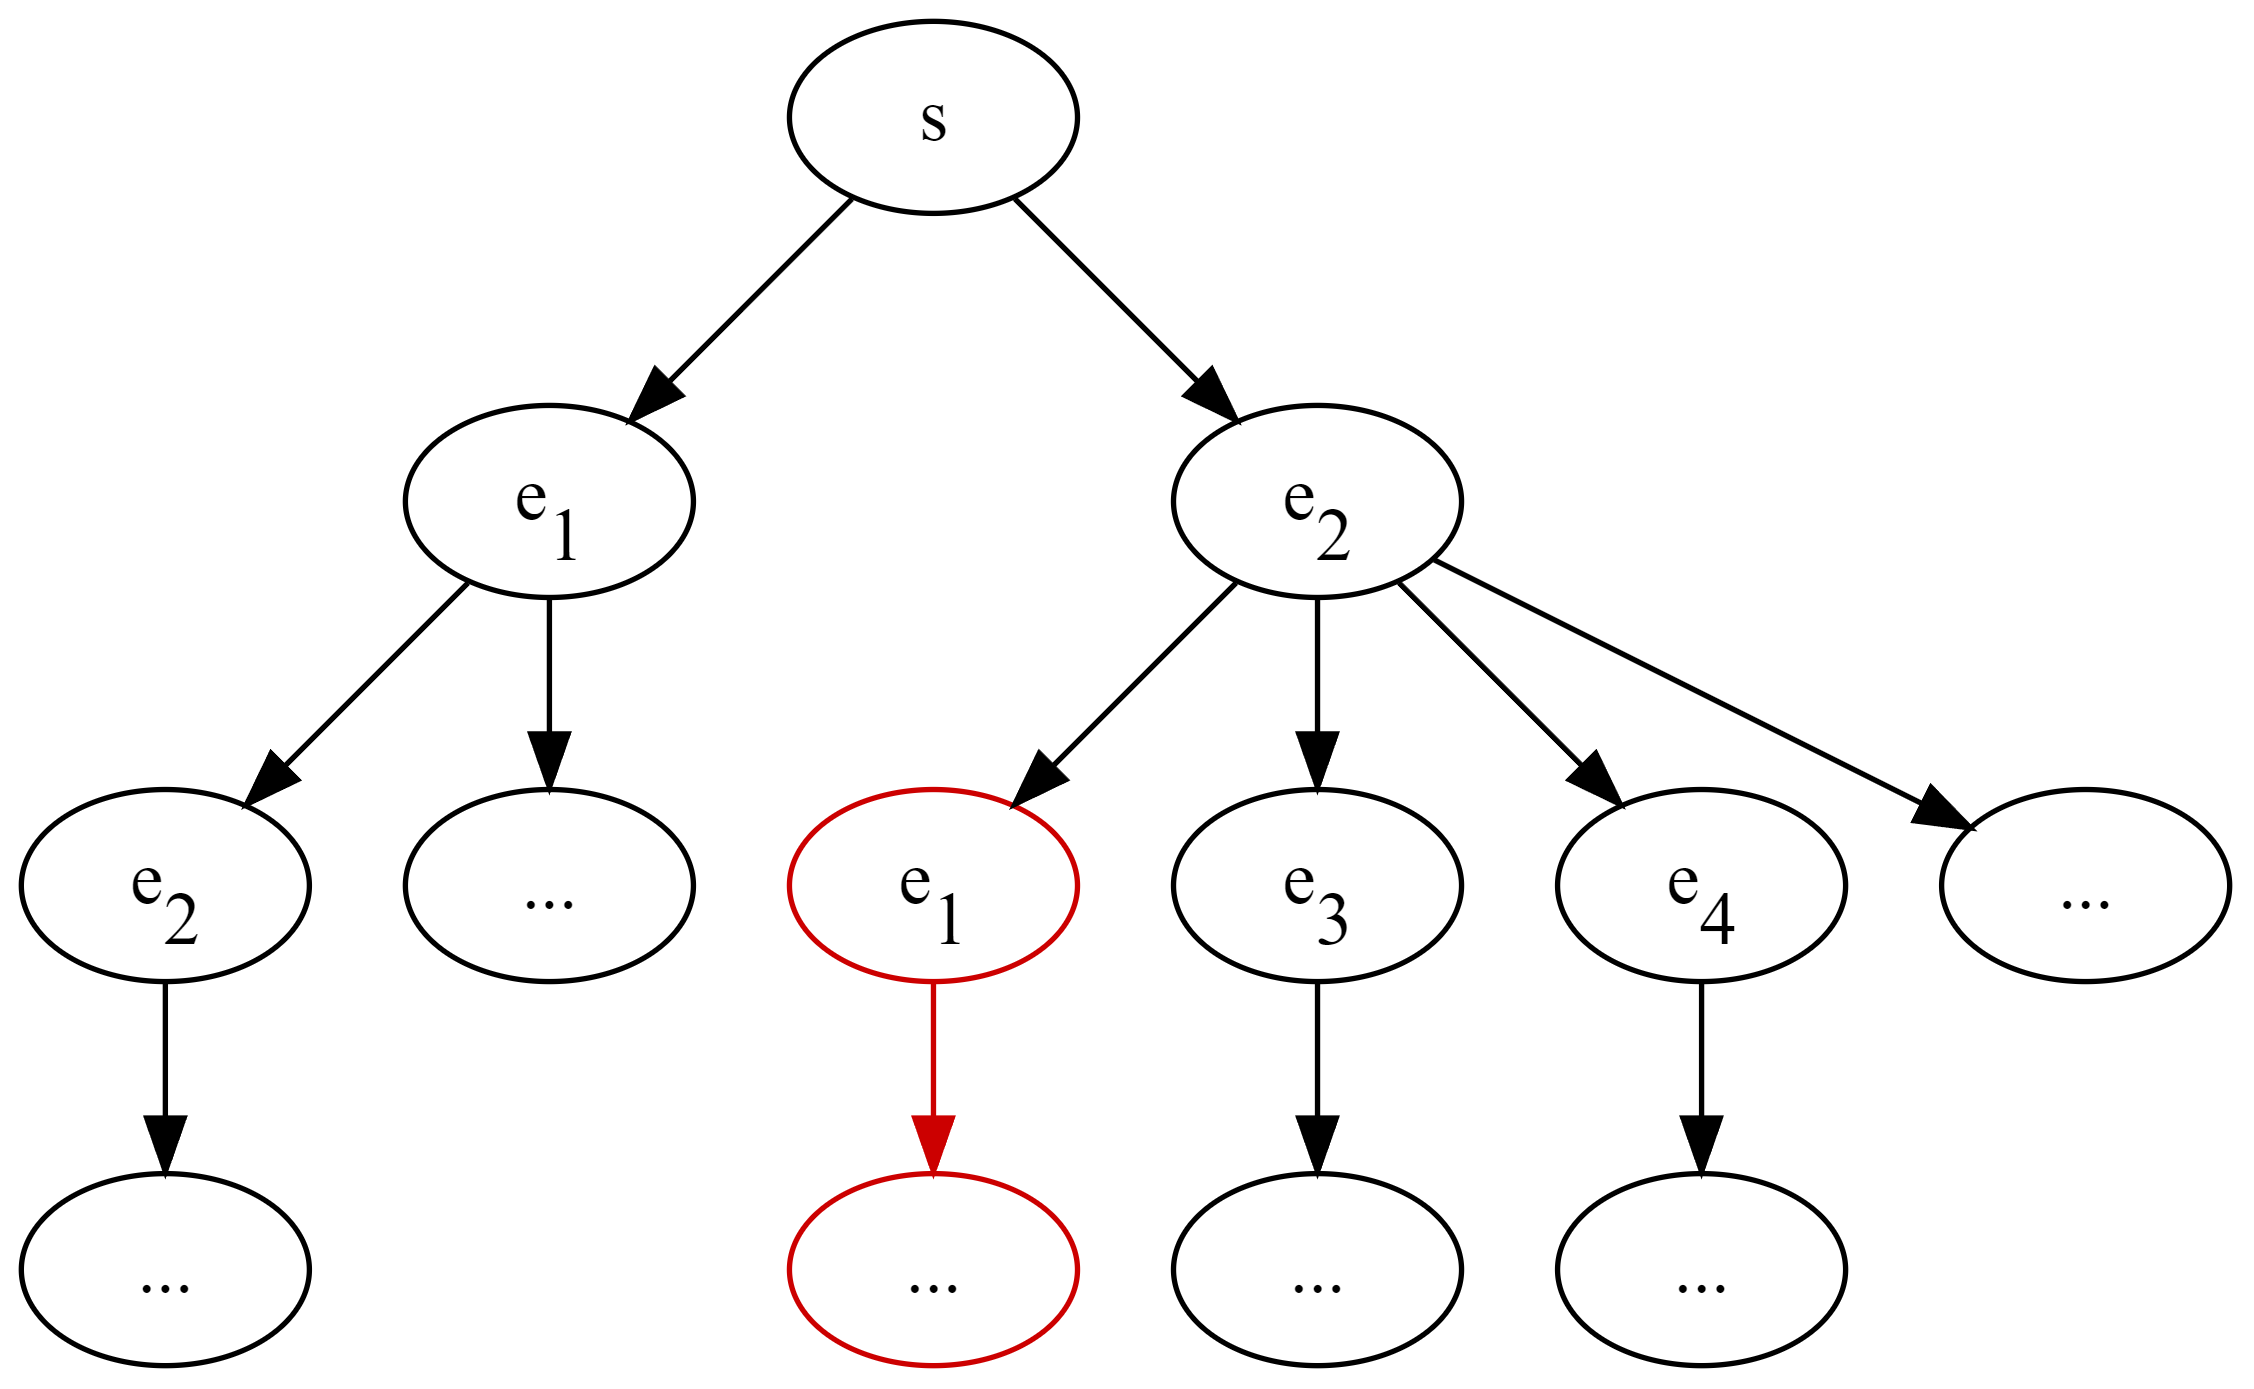
\includegraphics[width=0.85\linewidth]{img/DFS-graph.png}
    \caption{Example search tree for optimal solution completion}
    \label{fig:dfs-graph}
\end{figure}

Regular depth-first search marks each node in a graph as visited once it processes it, meaning that it will not come back to the same node again.
On the other hand, DFS used in the optimal completion cannot skip a potential takeoff just because it already encountered it at some previous time.
Consider a very simple example of a search tree in Figure \ref{fig:dfs-graph}, with a partial solution $s$ in the root node.
Let us start by inserting takeoff $e_1$, followed by takeoff $e_2$, as shown in the left branch.
Other takeoffs may also be inserted and evaluated, but that is irrelevant.
After the search in the left branch is completed and we have the best solution which contains $e_1$, the algorithm moves on to the right branch.
It starts by inserting the takeoff $e_2$, even though it was already visited in the left branch.
This is because the contexts are different -- in the left branch $e_2$ was explored in the context of an already inserted $e_1$, which most likely blocked some other potential takeoffs.
In the right branch, $e_2$ has an empty context because it is being inserted directly into $s$.
The next step would be to insert $e_1$.
However, that is unnecessary because we would get a partial solution $s \cup \{ e_1, e_2 \}$, which is a superset of the partial solution $s \cup \{ e_1 \}$, and that was already fully explored in the left branch.
Therefore, the red nodes in the tree are skipped during the search.

In order to keep track of which nodes can be safely skipped, thus reducing the search space, a set of visited takeoffs $V$ is used.
As mentioned, it does not contain all visited takeoffs, but only those that were already fully explored in the same context.
In practical terms, the visited set contains the left siblings of every ancestor of the currently observed node.
It does not contain the ancestors themselves, although including them would not make a difference. 
The ancestors cannot appear again in the currently explored subtree because they were already inserted into the current partial solution.
As an example, consider the takeoff $e_4$ in Figure~\ref{fig:dfs-graph}.
The visited set for that node would be $V = \{ e_1, e_3 \}$.
At the start of the search, $V$ is an empty set (line~\ref{alg:repair-line-optimal}).

In line~\ref{alg:repair-line-remove-visited} it can be seen that all takeoffs in the visited set $V$ are removed from $C$, the set of potential takeoffs that need to be explored.
Before starting a new recursive call, i.e., descending a level in the search tree, the takeoff $e$ is inserted into a copy of the current partial solution (line~\ref{alg:repair-line-recursion}).
The function result is the best solution in the searched subtree.
The function recursively calls itself for every child node (subtree) in the search tree, and tracks the best found solution.
It should be noted that the search tree is implicit and the set of potential takeoffs changes depending on which takeoffs were previously inserted.


\section{Simulated Annealing}\label{sec:simulated-annealing}

\textit{Simulated annealing} (SA) is an iterative, single-solution based metaheuristic algorithm inspired by the annealing process used in metallurgy, and the Boltzmann's law~\cite{Kirkpatrick/SA}.
This probabilistic technique is based on a Monte Carlo model which simulates energy levels in cooling solids~\cite{Misevicius/SA}.
The main idea behind simulated annealing is the possibility to accept non-improving solutions in order to escape from a local optimum, delaying the convergence and hopefully finding an ever better solution.

The most common method of updating the current solution $s$ is as follows:
if the generated neighboring solution $s'$ is better than the current solution, accept it;
if it is worse, accept it with a probability which depends on the current value of the control parameter $T \ge 0$, and the relative fitness $\Delta f = f(s') - f(s), \, \Delta f \le 0$.
For a maximization problem, the probability of acceptance of a non-improving solution is equal to $P(\Delta f) = e^{\Delta f / \, T}$.
This makes it less likely to accept far worse solutions which have a larger absolute value of $\Delta f$.

The control parameter $T$ represents the temperature in the real-world annealing process.
At high temperatures, the probability of acceptance will be higher, resembling random local search at extreme temperatures.
To facilitate convergence, the temperature is usually gradually reduced, intensifying the search in the process.
At the lowest temperature, $T = 0$, only improving solutions are accepted, resulting in a hill-climbing algorithm.

In the proposed algorithm, a homogeneous cooling schedule is used, slightly decreasing the temperature in every iteration, starting from the initial temperature $T_0$.
A simple geometric decrement function is used: $T \gets \beta \cdot T$.
The cooling factor $\beta \in [0, 1]$ determines the cooling speed, with a usual value very close to $1$.
Another popular decrement function is the \textit{very slow decrease}: $T \gets T \, / \left( 1 + \gamma \cdot T \right), \, \gamma \ge 0$.
However, at the beginning, this function reduces high temperatures far too rapidly, which is not suitable for use with very large absolute values of the objective function and its differences, as is the case in this optimization problem.
In order to have a meaningful probability of acceptance, an average $\Delta f$ and $T$ need to have roughly the same magnitude, making geometric decrease a better choice.

Simulated annealing is a part of local search, so it is integrated into Algorithm~\ref{alg:localsearch}.
At the beginning, the current temperature $T$ is set to the initial temperature $T_0$ (line~\ref{alg:localsearch-line-temp-init}).
In line~\ref{alg:localsearch-line-sa-accept}, the acceptance criteria are checked to see if the current solution should be replaced by the sampled solution.
Finally, the current temperature is updated in line~\ref{alg:localsearch-line-sa-end}, and the next iteration can commence.

State-of-the-art simulated annealing algorithms do not necessarily only decrease the temperature, but rather oscillate it~\cite{Misevicius/SA}\cite{Ma/InhomogeneousSA}.
This leads to reannealing (reheating), which can improve the found solutions.
However, it seems to have almost no effect on this particular problem, and results in approximately doubled execution time for local search.
Therefore, it was not included in the proposed algorithm.


\newcommand{\comment}[1]{}
\comment{

-- fig:dfs-graph --
https://dreampuf.github.io/GraphvizOnline
digraph G {
  e11[label=<e<SUB>1</SUB>>];
  e12[label=<e<SUB>1</SUB>>, color="#cc0000"];
  e21[label=<e<SUB>2</SUB>>];
  e22[label=<e<SUB>2</SUB>>];
  e3[label=<e<SUB>3</SUB>>];
  e4[label=<e<SUB>4</SUB>>];
  s -> e11;
  e11 -> e21 -> dots11;
  e11 -> dots1;
  s -> e22;
  e22 -> e12;
  e12 -> dots22 [color="#cc0000"];
  e22 -> e3 -> dots3;
  e22 -> e4 -> dots4;
  e22 -> dots2;
  dots1[label=<...>];
  dots2[label=<...>];
  dots3[label=<...>];
  dots4[label=<...>];
  dots11[label=<...>];
  dots22[label=<...>, color="#cc0000"];
}

}
